Macrocycles have recently gathered increased interest in medicinal chemistry as beyond rule-of-5 (bRO5) molecules. \cite{Driggers2008, Mallinson2012, Doak2014, Dougherty2017, Marsault2011, Abdalla2018, Marsault2017, Caron2021}
A key feature of these molecules is their conformational complexity that can be leveraged in drug design to target protein-protein interactions. \cite{ Chène2006, Janin2008, Jones13, Scott2016, Modell2016}
Such protein-protein interactions are typically characterized by large flat binding sites that are difficult to target with small molecules. \cite{Doak2016}
If the macrocycles are peptidic, their toxicity is often relatively low. \cite{Zorzi2017}
Most Food and Drug Administration (FDA)-approved macrocyclic drugs belong to natural products (e.g., erythromycin, tacrolimus) or peptides (e.g., sandostatin, eptifibatide). \cite{Giordanetto2014}
Peptidic or semipeptidic scaffolds bridge the gap between small molecules and biologics. An advantage of this molecule class is that they are relatively easy to synthesis and allow a broad choice of natural and non-natural amino acids required for rapid and thorough pharmacophoric exploration. 
The main challenge with peptides resides in their physicochemical and pharmacokinetics-ADME (absorption, distribution, metabolism, and excretion) properties. 
While cyclic peptides are typically more stable to proteases compared to their linear counterparts, their high polarity often translates into low bioavailability.\cite{Naylor2017, Fosgerau2015}
However, some cyclic peptides were found to cross cell membranes.\cite{Naylor2017, Wang2014, Nielsen2014} 
Developing tools and knowledge to optimize and better predict their structure–permeability relationship is, therefore, a requirement for the field. Such quest found inspiration in studies of the cyclic undecamer cyclosporine A, which is administered orally. 
One prominent structural feature of this natural macrocycle is the high number of N-methylated residues (7 out of 11) and its dynamic structural adaptation to its environment described as chameleonic behavior. \cite{Whitty2016, Danelius2020, Witek2017}
The effect of N-methylation on the permeability of cyclic hexa- and heptapeptides has been systematically investigated since the number and position of N-methylations may be beneficial or detrimental for permeability. \cite{Nielsen2014, Räder2018, White2011, Beck2012, Biron2008, White2011} 
%
Less explored are the N-alkylated glycines -- aka peptoids -- in which the side chain has been moved from the $\alpha$-carbon to the amide nitrogen. \cite{Schwochert2015} 
Similar to N-methylation, this modification removes one H-bond donor and removes one stereogenic center, and induces glycine-like secondary structures.
The peptoid amide also facilitates cis-trans isomerization compared to the corresponding N-methylation.\cite{Sui2007} 


More recently, the impact of the dynamics of macrocycles in response to their environment, which can range from polar in water, nonhomogeneous in the presence of its target, to lipophilic in the membrane, has been appreciated.\cite{Danelius2020, Witek2017, Riniker2019, Witek2019, Wang2021}
Studying macrocycles with computational methods leads to multiple criteria identified as being possibly essential for chameleonic behavior. Examples of these criteria are the presence of intramolecular H-bonds, 3D polar surface areas (3D-PSA), or kinetic Markov models as metrics for how macrocyclic structures yield polar atoms and rigidification of the backbone cycle into certain polar/apolar states. \cite{Witek2016, Witek2017, Tyagi2018, Witek2019, Wang2021}
A powerful tool to modulate the properties of peptidic macrocycles is the inclusion of a nonpeptidic tether unit.\cite{Marsault2007, Hoveyda2011, Roux2020} 
This tether can serve multiple purposes: in the context of a target interacting with a specific sequence, various tethers can be screened without modifying the peptide recognition sequence, while providing a simple handle for modulating affinity and pharmacokinetic properties. 
Small modifications in size, shape, or functional groups on the tether can dramatically influence on this kind of constrained system.\cite{Appavoo2019}
%
The relationship between structure and permeability is known to be elusive for this class of compounds, with small structural modifications often yielding permeability cliffs. \cite{Wang2014, Räder2018, Beck2012, White2011, Roux2020, Bockus2015, Hewitt2015, Rezai2006, Over2016}


To investigate the structural effects of a tether with a length of five atoms and the peptide-peptoid change on the compound permeability, our collaborators synthesized a collection of 36 semipeptidic macrocycles. \cite{Comeau2021, Roux2020}
The structure of the compounds was composed of a tripeptide tethered head-to-tail with a nonpeptidic linker (Figure \ref{fig:MolDes}). 
Two classes of modifications were explored: single peptoid replacement and regio- and stereocontrolled linker C-methylation. 
%
\begin{figure}[h!]
    \centering
    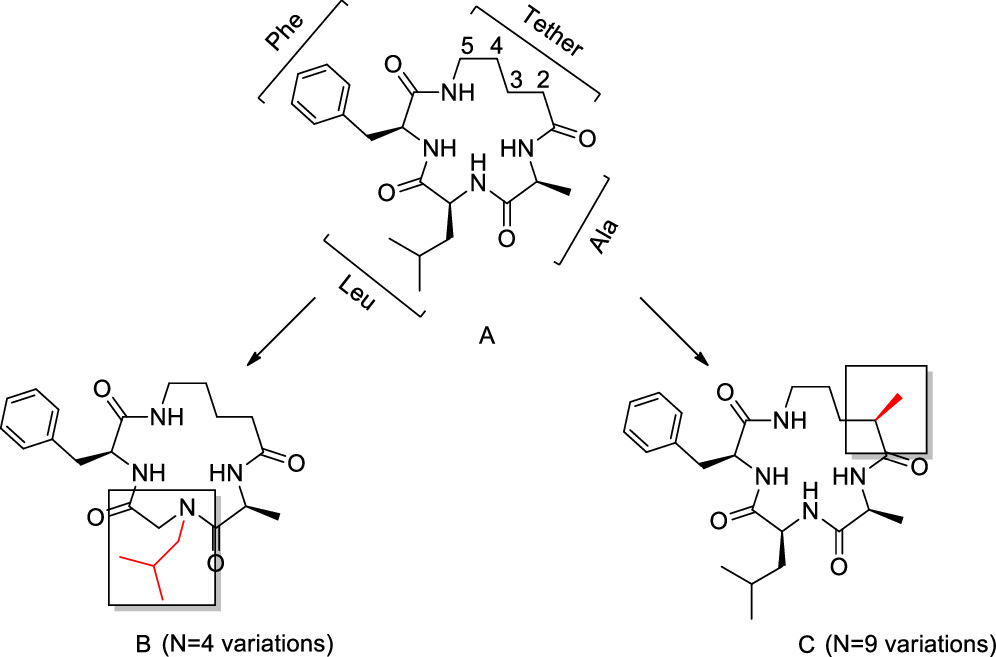
\includegraphics[width=\textwidth]{7_chapter_5/fig/intro/MoleculeDesign.jpeg}
    \caption{Synthesis strategy of our collaborators for model compound (\textbf{A}) and two types of modifications: Nala, Nleu, and Nphe peptoids (\textbf{B} showing Nleu) and regio/stereocontrolled C-methylation (\textbf{C} showing 2R methylation).\cite{Comeau2021}}
    \label{fig:MolDes}
\end{figure}

\begin{figure}[h!]
    \centering
    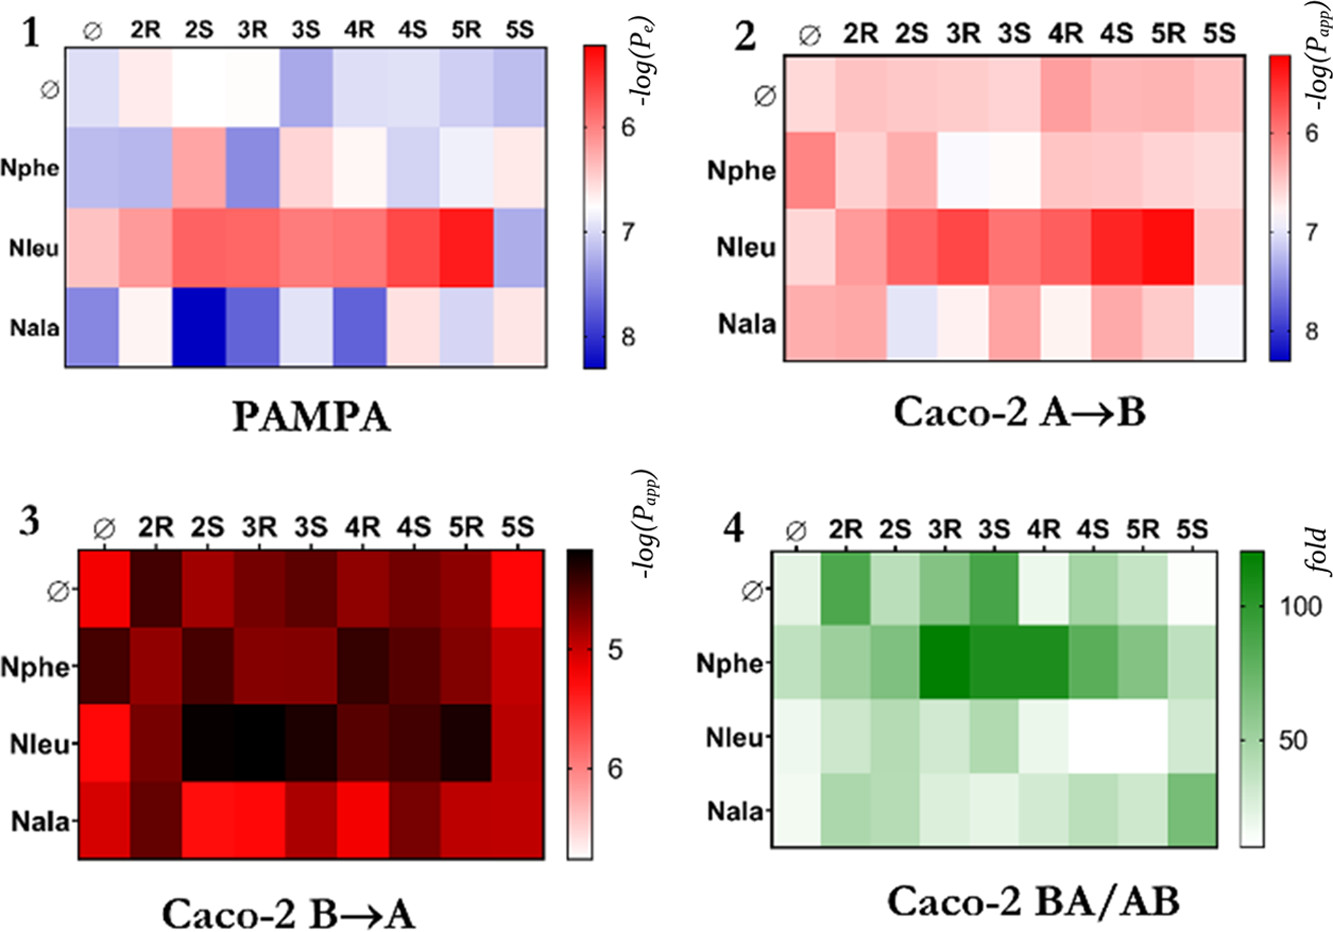
\includegraphics[width=\textwidth]{7_chapter_5/fig/intro/pampa.jpeg}
    \caption{Permeability results in the form of heatmaps. For heatmaps 1–3, the values are expressed as $−log(P_{\text{app}})$, so lower values mean higher permeability (in order of increasing permeability: blue, white, red, and black). Heatmap 4 shows the BA/AB ratio, which represents a measure of efflux.}
    \label{fig:permAssays}
\end{figure}
The passive permeability of the resulting macrocycles was measured by our collaborators in the parallel artificial membrane permeability assay (PAMPA) and their cellular permeability in the Caco-2 assay\cite{Di2015} (Figure \ref{fig:permAssays}).\cite{Comeau2021}

%
\begin{figure}
    \centering
    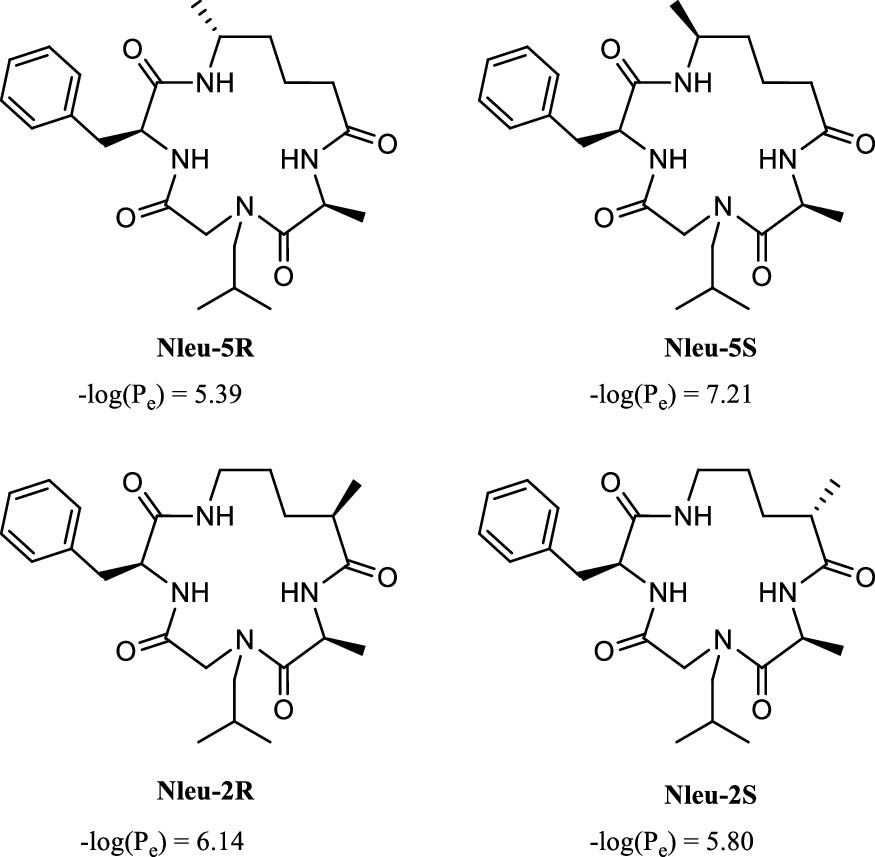
\includegraphics[width=\textwidth]{7_chapter_5/fig/intro/permCliffMols.jpeg}
    \caption{Four semipeptidic macrocycles were selected from the collection. In contrast to the pair Nleu-2R/S (bottom), the pair Nleu-5R/S (top) behave significantly  different in the permeability assays. All molecules were  studied with experimental NMR analysis and molecular dynamics (MD) simulations in a polar and apolar environment.}
    \label{fig:permCMols}
\end{figure}
Based on the permeability data, we selected two pairs of diastereomers that differ only by their stereochemistry of the tether methyl group (Figure \ref{fig:permCMols}). While one pair (Nleu-5R/S) differs greatly in their passive permeability behavior, the second one (Nleu-2R/S) does not. 
Prior studies on cyclosporine A showed that the conformational behavior of cyclic peptides in the context of membrane permeability can be studied by performing extensive molecular dynamics (MD) simulations in apolar and polar environments (e.g., chloroform and water) to mimic the behavior outside and inside a membrane. \cite{Witek2016,Witek2017, Witek2019, Wang2021}
Therefore, we carried out MD simulations of each of the four selected macrocycles in water and chloroform. The simulations results were validated by comparing to solution NMR measurements of the compounds. \cite{Balazs2019}
Finally, we used different metrics such as torsional angles, hydrogen-bond formation, and 3D-PSA\cite{Sebastiano2018} to assess and compare the conformational behavior of the compounds. 